% app2.tex (file to switch to appendix mode)

\chapter[\celloPiece]{}

\vspace*{3cm}
\begin{center}
\textsc{for solo violoncello}

\vspace*{3.5cm}

\HRule{0.5pt}


\LARGE \textbf{\uppercase{\celloPiece}}
\HRule{2pt}

\vspace{1.3cm}

\normalsize October, 2019
\date{}

\vspace*{5\baselineskip}

Rhys Gray

\end{center}
\newpage
\newpage

\section*{Program Notes}
\celloPiece\space is a piece for solo violoncello, written to explore \hyperref[sec:multiphonics]{multiphonics}. 

Multiphonics are achieved through clusters of close harmonic nodes, and by playing a harmonic close to the highest partial.
  Note that not all of these pitches will actually sound in practice.
  
  Multiphonics are notated as a harmonic position using a diamond notehead, with an `M' above the note to be fingered.
  Where the string used is ambiguous, it is notated below the sounding pitch as a small, bracketed notehead.
  Precise tuning is given in cents, and unless otherwise notated, is intended for the first note that the multiphonic is attached to.\footnote{100 cents is equal to a semitone. Therefore, +51c is roughly equal to half a semitone sharp. Cents have been used due to their precision compared to more granular accidentals such as the quartertone sharp.}
  The theoretical sounding pitches are given in a bracketed staff above the main stave.
  % Above the sounding pitches, the sounding partials are given (i.e. M IV [4th + 13th + 9th + 15th + 5th]).

  The bow should exert slightly more pressure than usual and should be drawn with a consistent speed which should be slower than for harmonics.
  The location of the bow can encourage or discourage upper or lower partials, and experimentation should be done during the practice of this work to achieve the pitches desired.

\section*{Notation}
\begin{itemize}
  \item Multiphonics are denoted with a diamond notehead, marked with an M (see \autoref{fig:multiphonicsBassExample} for an example). 
  \begin{itemize}
    \item Precise tuning in cents (i.e. +41c) is provided to help the performer pitch the fingering required for the multiphonic to be produced.
    \item The multiphonic resultant pitches are notated at pitch in the \emph{suono reale} stave, with the cents tuning of the resultant pitches to the left or right of the notes.
  \end{itemize}
    \item Arrows denote gradual transitions to the technique that the arrow is pointing to.\begin{itemize}
      \item Arrows between notes denote transitions between the types of notes (i.e.\ \emph{normale} to harmonic finger pressure.)
    \end{itemize}
    \item n denotes \emph{normale}.
    \item sp denotes \emph{sul ponticello}.
    \item msp denotes \emph{molto sul ponticello}.
    \item similarly, st denotes \emph{sul tasto}, and mst denotes \emph{molto sul tasto}
\end{itemize}

\newpage\label{app:celloPiece Score}
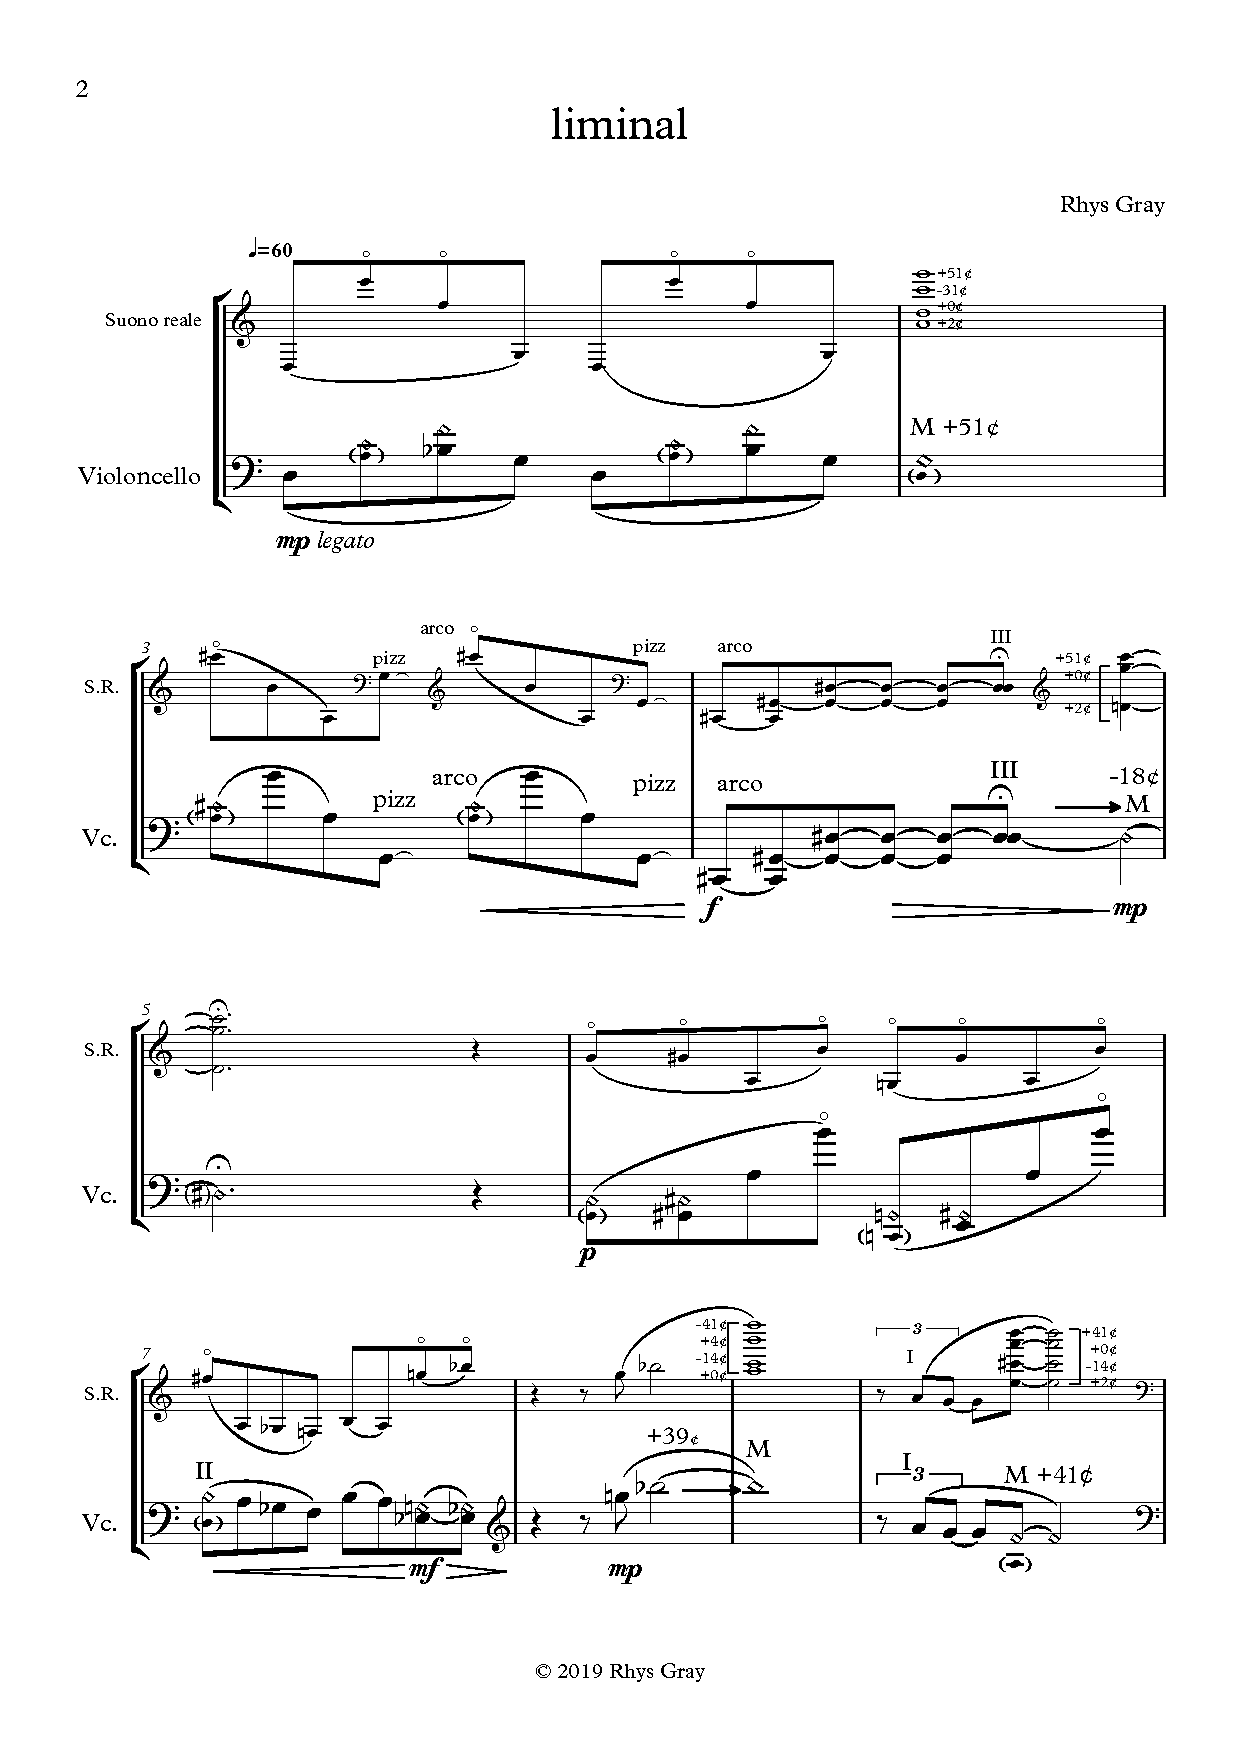
\includepdf[pages=-,pagecommand={}]{resources/compositions/violoncello.pdf}